\documentclass[a4paper]{article}

\usepackage{amsmath}
\usepackage{listings}
\usepackage{amsfonts}
\usepackage{amssymb}
\usepackage{graphicx}
\usepackage{titling}
\usepackage[utf8]{inputenc}
\usepackage[english]{babel}
\usepackage{fancyhdr}
\usepackage{lastpage}
\usepackage{textcomp}
\usepackage{hyperref}
\usepackage{float}
\usepackage{color, soul}

\addtolength{\oddsidemargin}{-.875in}
\addtolength{\evensidemargin}{-.875in}
\addtolength{\textwidth}{1.75in}
\addtolength{\topmargin}{-.875in}
\addtolength{\textheight}{1.75in}

\title{\Huge Medical Technologies Synopsis \vspace{1cm}}
\author{MrRattoSpaccio, Lolinear}
\date{May 23rd 2019}
\setcounter{page}{0}
\pagestyle{fancy}
\fancyhf{}

\fancyfoot[C]{Page \thepage \hspace{1pt} of \pageref{LastPage}}

\begin{document}
\maketitle
\thispagestyle{empty}
\pagebreak
\tableofcontents

\section{Introduction}
\subsection{Tipologie di Ingegneri biomedici}
\begin{description}
    \item[Clinici] Lavorano negli ospedali, essi aiutano altri operatori degli
    ospedali a scegliere l'apparecchiatura più giusta per l'assistenza ai 
    pazienti. Si occupano anche di assicurare che le apparecchiature siano
    sicure ed affidabili.
    \item[Progetto e Ricerca] Lavorano nelle grandi aziente, progettano sistemi
    per il monitoraggio continuo dei pazienti critici, organi artificiali, o 
    schemi e procedure per somministrare terapie in modo sicuro ed efficace.ù
    \item[Riabilitazione] Utilizzano la tecnologia ed i calcolatori per 
    aiutare le persone con disabilità e migliorare la qualità della loro vita.
    \item[Ricerca (Scuole)] Lavorano nei laboratori di ricerca di scuole di 
    medicina o università, acquisendo nuove conoscenze sugli organismi viventi.
    \item[Vari] Alcuni studiano cellule ed insiemi di molecole, alcuni organi
    composti da insiemi di cellule, altri creano modelli matematici che 
    descrivono le funzionalità del corpo. Altri ancora studiano materiali
    artificiali necessari alla creazione di dispositivi medicali. 
\end{description}
\subsection{Dispositivi medicali (DM)}
\subsubsection{Definizione}
\paragraph{Completa}
S’intende per dispositivo medicale, qualunque strumento, apparecchio, 
apparecchiatura, materiale, prodotto, all’eccezione dei prodotti d’origine 
umana, o altro articolo usato da solo o in combinazione, compresi gli accessori
e software necessari per il suo funzionamento, destinato dal fabbricante ad 
essere impiegato sull'uomo per scopi medici e la cui azione principale voluta 
non si ottiene con mezzi farmacologici o immunologici o metabolici, ma dove 
la funzione può essere assistita da tali mezzi.
\paragraph{Concisa}
Ogni prodotto utilizzato per scopi medici che non è, né un medicamento, né un 
prodotto biologico, è identificabile con la terminologia di Dispositivo Medico.
\subsubsection{Utilizzi}
\begin{itemize}
    \item Diagnosi, prevenzione, controllo, terapia o attenuazione di una 
    malattia
    \item Diagnosi, controllo, terapia, attenuazione o compensazione di una 
    ferita o di un handicap
    \item Studio, sostituzione o modifica dell'anatomia o di un processo 
    fisiologico
    \item Controllo e gestione del concepimento
\end{itemize}
\subsubsection{Categorie}
\begin{description}
    \item[Impiantabili attivi (DMIA)] Pacemaker, defibrillatori, pompe 
    \item[Diagnostica in Vitro (DM DIV)] Reagenti per le diagnosi
    \item[Compensazione degli handicap] Sedia a rotelle, apparecchi acustici
    occhiali, ecc.
    \item[Su misura] protesi dentarie, plantari ortopedici, ecc.
    \item[Diagnostica/Pratiche Terapeutiche/Supporto Vitale] Scanner, macchina
    per la dialisi, radioterapia, monitor di sorveglianza, defibrillatori
    esterni
    \item[Monouso] Aghi, bende, siringe, ecc.
    \item[Impianti chirurgici non attivi] protesi d'anca, valvole cardiache, ecc.
\end{description}
\subsection{Dispositivi Medicali Impiantabili Attivi (DMIA)}
Dispositivi medici che sono progettati per essere impiantati totalmente o in 
parte nel corpo umano... e che dipendono per il loro corretto funzionamento 
da una fonte d’energia elettrica o da qualsiasi altra fonte d’energia diversa 
da quella prodotta direttamente dal corpo umano o dalla gravità.
\subsection{Dispositivi Medicali di Diagnostica In Vitro (DM DIV)}
Prodotti, reagenti, materiali, strumenti... destinati ad essere utilizzati in 
vitro per l'esame di campioni provenienti dal corpo umano con lo scopo di 
fornire informazioni relative a una condizione fisiologica o patologica.
\subsection{Classificazione dei DM}
I dispositivi medici, eccetto i DMIA e i DM DIV sono classificati in 4 classi:
\begin{itemize}
    \item Classe I $\to$ Rischio potenziale debole (Lenti da vista, 
    Stetoscopi, ecc.)
    \item Classe IIa $\to$ Rischio potenziale moderato (Lenti a contatto, 
    Catateri urinari, ecc.)
    \item Classe IIb $\to$ Rischio potenziale elevato (Laser chirurgici, 
    Cemento osseo, ecc.)
    \item Classe III $\to$ Rischio potenziale critico (Stent, valvole cardiache, 
    ecc.)
\end{itemize}
Tutti i DMIA sono classificati come Classe III.
\subsubsection{Regole di classificazione}
\begin{itemize}
\item Il periodo d’utilizzo o più precisamente la durata in cui il dispositivo
è in continuità in contatto col paziente
\item L’invasività: il dispositivo è invasivo o no, e se lo è, qual è il grado
d’invasività (penetrazione attraverso un orifizio del corpo o tramite 
impianto chirurgico)
\item La possibilità o meno di riutilizzo
\item L’obiettivo terapeutico o diagnostico
\item La dipendenza da una fonte d’alimentazione diversa da quella umana
\item La parte del corpo che viene a contatto con il dispositivo medico: sistema circolatorio centrale,
sistema nervoso centrale, ecc.
\end{itemize}
\paragraph{Classe I}
Strumenti chirurgici riutilizzabili, dispositivi medici non invasivi, 
dispositivi medici invasivi per uso temporaneo, ecc.
\paragraph{Classe IIa}
Dispositivi medici di classe I sterili e/o con funzione di misurazione, lenti a 
contatto, protesi dentarie, ecc.
\paragraph{Classe IIb}
Dispositivi medici impiantabili a lungo termine, ecc.
\paragraph{Classe III}
Dispositivi medici impiantabili a lungo termine in contatto con il cuore, il 
sistema circolatorio centrale o il sistema nervoso centrale, i dispositivi 
medici impiantabili riassorbibili, protesi al seno, protesi d'anca, protesi
di ginocchio, ecc.
\subsection{Prodotti di Frontiera}
Si parla di prodotti combinati o di frontiera:
\begin{itemize}
    \item Quando un DM forma con un farmaco un prodotto un prodotto integrato.
    Ad esempio le siringhe pre-riempite.
    \item Quando un DM incorpora una sostanza che, utilizzata sola, può essere
    considerata come un farmaco. Ad esempio il cemento osseo con antibiotico.
\end{itemize}
Il prodotto combinato è considerato come un farmaco o un dispositivo medico in 
base all'azione principiale prevista.
\subsection{Considerazioni e Prospettive nel campo}
Troppo spesso l'utilizzo delle tecnologie medicali o viene promosso con
eccessiva facilità senza averne valutato adeguatamente le implicazioni o viene 
limitato dai timori derivanti dall’incertezza circa gli esiti e le conseguenze
del loro impiego. \\
La figura tecnica di riferimento per le tecnologie sanitarie, quale l’ingegnere 
biomedico, deve compiere uno sforzo di ampliamento del suo background formativo
e focalizzare maggiore attenzione sugli aspetti di valutazione dei rischi, dei 
costi e dei benefici delle nuove tecnologie sanitarie.

\section{Organizzazione del corpo umano, cellule e tessuti}
\paragraph{Anatomia} La scienza che studia la struttura di un corpo e le 
relazioni tra le sue parti.
\paragraph{Fisiologia} La scienza che studia come funzionano le parti di un
organismo.
\subsection{Livelli di organizzazione ed apparati del corpo}
\begin{enumerate}
    \item Livello della chimica (o molecolare): include gli atomi e le molecole
    \item Livello cellulare: le cellule sono le unità strutturali e funzionali 
    di base dell’organismo
    \item Livello dei tessuti: i tessuti sono costituiti da gruppi di cellule 
    che svolgono una funzione particolare
    \item Livello degli organi: i diversi tipi di tessuti si uniscono a formare 
    gli organi
    \item Livello dei sistemi e degli apparati: i sistemi sono costituiti da 
    organi con la medesima origine embriologica; gli apparati possono avere 
    struttura o derivazione embriologica diversa
    \item Livello dell’organismo
\end{enumerate}
\begin{figure}[H]
    \centering
    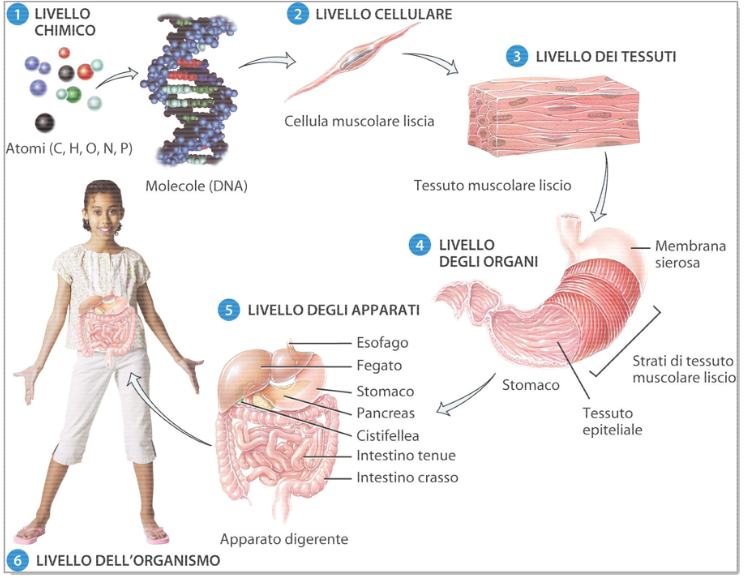
\includegraphics[scale=0.3]{figures/levels.png}
    \caption{Livelli di organizzazione}
\end{figure}
\subsection{Processi della vita}
\begin{description}
    \item[Metabolismo] L'insieme di tutti i processi chimici che avvengono nel
    corpo, tra cui la scissione di molecole e la loro sintesi
    \item[Reattività] La capacità di rilevare e di rispondere ai cambiamenti
    dell'ambiente interno/esterno
    \item[Movimento] Gli spostamenti di tutto il corpo, compresi gli organi, le
    cellule e gli organuli cellulari
    \item[Accrescimento] L'aumento delle dimensioni corporee
    \item[Differenziazione] Il processo in cui le celle indifferenziate si
    specializzano
    \item[Riproduzione] Intesa come sintesi di nuove cellule e generazione di
    un nuovo individuo
\end{description}
\subsection{Omeostasi}
L'omeostasi è il mantenimento della stabilità delle condizioni del corpo. 
Essa:
\begin{itemize}
    \item Garantisce il funzionamento cellulare
    \item Interviene per ripristinare le condizioni di stabilità 
    controbilanciando i cambiamenti interni/esterni
    \item Varia entro un ristretto ambito compatibile coi processi vitali delle
    cellule
\end{itemize}
Esistono dei sistemi di feed-back che permettono il mantenimento dell'omeostasi,
rappresentati da un ciclo di eventi dove la condizione del corpo viene 
continuamente monitorata, valutata e modificata. Così facendo si ottiene una
condizione controllata, perturbabile da uno \textbf{stimolo}.

\subsubsection{Sistemi di feed-back}
Un sistema di feed-back è costituito da:
\begin{description}
    \item[Recettore] Struttura che rileva i cambiamenti che avvengono in una 
    condizione controllata e invia tale informazione o input a un centro di 
    controllo
    \item[Centro di controllo] Valuta l’input ricevuto e invia comandi in 
    uscita all’effettore per il ripristino della condizione controllata
    \item[Effettore] Struttura che riceve l’output e produce una risposta 
    che modifica la condizione controllata
\end{description}

\section{Aspetti socio-economici, leggi, e norme}
\subsection{Generalità e definizioni}
Definizione di \textbf{dispositivo medico}:
\begin{quote}
    \centering
    Uno strumento, un apparecchio, un impianto, una sostanza, o altro prodotto 
    usato da solo o in combinazione, compreso il software informatico impiegato 
    per il suo corretto funzionamento, e destinato dal fabbricante ad essere 
    impiegato nell'uomo a scopo di:
    \begin{itemize}
        \item diagnosi, prevenzione, controllo, terapia o attenuazione di una 
        malattia (tomografo)
        \item diagnosi, controllo, terapia, attenuazione o compensazione di 
        una ferita o di un handicap (filo per suture)
        \item studio, sostituzione o modifica dell'anatomia o di un processo 
        fisiologico (protesi)
        \item intervento sul concepimento (profilattico)
    \end{itemize}
    Un dispositivo medico non deve esercitare la sua azione principale nel o 
    sul corpo umano con mezzi farmacologici o immunologici, né mediante processo 
    metabolico, anche se la sua funzione può essere coadiuvata da tali mezzi. 
\end{quote}
Definizione di \textbf{malattia}:
\begin{quote}
    \centering
    \hl{Alterazione dello stato fisiologico e psicologico dell'organismo}, capace di 
    ridurre, \hl{modificare negativamente} o persino eliminare le funzionaità normali 
    del corpo. Il concetto di malattia deve essere inteso come status e condizione 
    \hl{potenzialmente reversibile} attraverso l'applicazione di una terapia; questa 
    caratteristica di reversibilità é alla base del dibattito, sempre aperto, sul 
    fatto che alcuni stati dell'organismo dovuti alla genetica, come ad esempio la 
    condizione di sterilità, non siano definibili come malattia.
\end{quote}
\subsection{Aspetti socio-economici}
Nella medicina moderna, il problema non sembra più essere solo la guarigione e il 
recupero da una malattia ma anche quello di intervenire in anticipo e in qualche 
modo affinché la malattia o il semplice malessere non abbia neanche la possibilità 
di manifestarsi.

Condizioni legate al normale decorso della vita dell'organismo (menopausa, vecchiaia), 
o alla condotta di vita della persona (stress da lavoro), sono diventate vere e proprie 
patologie, con farmaci, terapie e strumenti atti al trattamento dei sintomi. Questo non 
può che avere profondi riflessi sull'estensione dei compiti ch evengono affidati alla 
medicina, spesso sulla base delle sue stesse proposte.

\subsection{Leggi e norme}
Il marchio CE, secondo il "nuovo approccio", definisce delle direttive da rispettare per 
l'ottenimento di un marchio CE che permette il libero scambio dei prodotti all'interno 
di una comunità. Le direttive introducono il seguente concetto fondamentale: 
\begin{quote}
    \centering
    Il fabbricante ha il dovere di rendere i propri prodotti sicuri e deve poter 
    dismostrare di aver fatto tutto il possibile per rendere i prodotti sicuri per poter 
    meglio definire, dai punti di vista costruttivo e della sicurezza, il libero scambio 
    interno dei prodotti di fabbricazione.
\end{quote}
Le direttive sono atti comunitari che:
\begin{quote}
    \centering
    vincolano lo stato membro per quanto riguarda il risultato da raggiungere, salva 
    restando la competenza degli organi nazionali in merito alla forma ed ai mezzi con 
    i quali raggiungere tali risultati.
\end{quote}
Le direttive non sono direttamente obbligatorie e vincolanti negli stati membri, ma sono 
implementate dagli organi nazionali competenti.
\subsection{Direttiva-tipo}
Nel nuovo approccio, una direttiva-tipo é strutturata secondo i seguenti criteri:
\begin{description}
    \item[Campo di applicazione]: prodotti coperti, rischi da evitare
    \item[Clausola generale di immissione sul mercato]: responsabile della sicurezza del 
    prodotto e della sua immissione sul mercato (usualmente il fabbricante o l'importatore)
    \item[Elenco dei requisiti essenziali di sicurezza]: sufficientemente precisi da 
    permettere la costituzione di obbligihi sanzionabili dagli stati membri
    \item[Clausola di libera circolazione]: garantisce la libera circolazione del prodotto
    marcato CE ed é la "ricompensa" per tempo e risorse investite per la certificazione
    \item[Norme armonizzate]: riferimento alle norme tecniche e di sicurezza elaborate 
    dagli organismi di normalizzazione europei
    \item[Procedure di certificazione]: procedure a cui vanno sottoposti i prodotti per 
    dimostrarne la conformità ai requisiti essenziali per l'apposizione della marcatura 
    CE
    \item[Fascicolo tecnico]: documentazione tecnica dimostrante la conformità del prodotto    
\end{description}
La marcatura CE é una sorta di "logo" che attesta la conformità del prodotto ai requisiti 
minimi di sicurezza della direttiva.\newline
\textbf{Il marchio CE é obbligatorio per i dispositivi medici.}
\subsection{Direttive medicali}
\subsubsection{Direttiva 93/42/CE "dispositivi medicali"}
\begin{description}
    \item[Considerazioni]: Considerando che occorre adottare provvedimenti nel contesto 
    del mercato interno, caratterizzato da uno spazio senza frontiere interne nel quale 
    sia assicurata la libera circolazione delle merci, delle persone, dei servizi, e dei 
    capitali.
    \item[Articoli]: 
    \begin{description}
        \item[Art.1 - Requisiti essenziali]: cosa occorre rispettare per poter garantire 
        la sicurezza del prodotto.
        \item[Art.5 - Rinvio alle norme]: riferimenti alle norme specifiche di prodotto.
        \item[Art.9 - Classificazione]: classe di pericolosità del dispositivo medico (big number = big bad):
        \begin{itemize}
            \item Classe I
            \item Classe IIa
            \item Classe IIb
            \item Classe III
        \end{itemize}
        \item[Art.11 - Valutazione della conformità]: descrive nel dettaglio il percorso 
        da seguire per dimostrare che il prodotto in questione é conforme aui requisiti 
        essenziale e che quindi, opportunamente marcato col simbolo CE, può essere posto 
        in commercio nella comunità. Per un dispositivo di classe I, un fascicolo tecnico 
        é spesso sufficiente, per dispositivi di classe più elevata diventa notevolmente 
        più complesso.
        \item[Art.16 - Organismi notificati] 
    \end{description} 
\end{description}
\subsubsection{Direttiva 2007/47/CE}
\begin{description}
     \item[Fascicolo tecnico]
     \begin{description}
        \item[Checklist requisiti essenziali]: prove che tutti i requisiti essenziali sono 
        soddisfatti.
        \item[Introdurre riferimenti alle 2007/47/CE]: riportare tutta la documentazione 
        utilizzata come riferimento in fase di progettazione.
        \item[Dati clinici]: dimostrazione della conformità delle includere una valutazione 
        clinica.
        \item[Modifica analisi ed accettabilità del rischio]: rischi associati all'ergonomia 
        del prodotto.
        \item[Revisione tempi di conservazione]: conservazione della documentazione 
        prolungata a 15 anni per alcuni dispositivi impiantabili.
        \item[Revisione labelling e dichiarazione di conformità]
        \item[Revisione istruzioni per l'uso]: identificare il dispositivo ed il contenuto 
        della confezione.  
     \end{description}
     \item[Procedure]
     \begin{description}
         \item[Controllo sui terzi]: dimostrare controlli adeguati nei confronti di soggetti 
         terzi.
         \item[Monitoraggio after-marketing]: l'obbligo di comunicazione al Ministero il 
         verificarsi di incidenti
         \item[Diversa valutazione della conformità]: qualora non si ritenga opportuna 
         la dimostrazione della conformità ai requisiti essenziali va debitamente 
         provata l'adeguatezza della dimostrazione della conformità ai requisiti 
         essenziali.
     \end{description}  
\end{description}
\section{Controllo qualità}
\subsection{Introduzione}
La misura della \textbf{qualità} indica una misura delle caratteristiche o delle 
proprietà di una entità in confronto a quanto ci si attende da una tale entità.\newline
L'uso che si intende fare dell'entità é importante.
\subsection{Evoluzione del concetto di qualità}
Il rilevante compito di diffusione della cultura della qualità é stato assolto dall'ISO.\newline
\begin{description}
    \item[ISO 29000:1987]: soluzioni preconfezionate ritenute fondamentali. L'utilizzo 
    delle prescrizioni rappresenta per l'azienda un'occasione per analizzare alcuni 
    aspetti della propria organizzazione. Il modello proposto si adatta a qualsiasi realtà
    produttiva. Importante la distinzione tra azione correttiva e azione preventiva. La 
    prima migliora o potenzia un aspetto del sistema qualità che ha prodotto una 
    non-conformità. La seconda agisce in seguito allo scopo di prevenire non-conformità 
    ancora non presentatesi.
    \item[ISO 9000-1994]: evolutosi dall'ISO 29000, pone come riferimento centrale la 
    figura del cliente, figura che non rappresenta solo l'utilizzatore finale ma anche 
    altre entità del processo realizzativo ("cliente interno"). L'attenzione é posta 
    sui rapporti interaziendali. La possibilità offerta ad un reparto-cliente di esprimere 
    un livello di soddisfazione verso un servizio/prodotto fornito da un reparto fornitore, 
    aiuta ad uno scambio culturale/professionale più ricco ed efficiente.
    \item[ISO 9001:2000 e ISO 9001:2008]: focus sul \textbf{miglioramento continuo} 
    dei processi aziendali, tramite un processo gestionale integrato in cui il 
    coinvolgimento di tutto il personale, la pianificazione , la documentazione 
    dell'attività, e l'atteggiamento volto al miglioramento continuo, diventano i 
    cardini del nuovo modello di gestione.
\end{description}
\subsection{Qualità di un prodotto e/o servizio}
La ISO 9000 ha avuto il merito di spostare l'attenzione dalla qualità del prodotto/servizio 
all'insieme dei processi aziendali che contribuiscono alla sua realizzazione. \hl{Solo da 
processi ben gestiti e tenuti sotto controllo nascono buoni prodotti e servizi}.\newline
Il concetto di qualità dipende da
\begin{itemize}
    \item chi fornisce il prodotto
    \item chi lo commissiona e/o lo utilizza
\end{itemize}
Soggetti o elementi base della qualità per
\begin{description}
    \item[prodotti/servizi]:
    \begin{itemize}
        \item chi \textbf{esprime} i requisiti, usualmente il cliente e/o l'utilizzatore
        \item chi \textbf{fornisce} il prodotto/servizio: impresa, istituzione, \dots
        \item il \textbf{prodotto} deve avere una qualità definita (conformità a standard o specifiche)
        \item fattori \textbf{percepibili} da parte del cliente
    \end{itemize}
    \item[i processi relativi]:
    \begin{itemize}
        \item il \textbf{processo aziendale} deve essere misurabile tramite 
        \textbf{indicatori di prestrazione (PKI)} e \textbf{indicatori della qualità oggettivi}
        \item il \textbf{monitoraggio nel tempo} é strumento fondamentale per valutare 
        bontà e margini di miglioramento dei processi. La produzione a \textbf{"zero difetti"}
        é spesso economicamente insostenibile
        \item Definizione delle specifiche deve essere concordata da tutte le parti in causa, 
        e quest'ultime sono tenute a mantenere l'incarico per tutta la durata del progetto
    \end{itemize}
    \item[prodotti, servizi, progetti e processi]:
    \begin{itemize}
        \item capacità di raggiungere gli obiettivi stabiliti (\textbf{efficacia}) e 
        utilizzando al meglio le risorse a disposizione (\textbf{efficienza})
        \item un documento che riassume le caratteristiche del prodotto/servizio, ed é 
        solitamente il contratto, la specifica, la convenzione, la carta dei servizi, 
        o il piano della qualità
    \end{itemize} 
\end{description}
\subsection{Le richieste del cliente}
Secondo lo schema della qualità alla sorgente, ogni caratteristica deve essere definita 
e messa sotto controllo ilprima possibile lungo il processo che porta al cliente. 
Prima di iniziare a lavorare bisogna elaborare una strategia organizzativa e definire 
gli obiettivi sulla base delle esigenze dell'utilizzatore.\newline
Il punto di partenza di ogni prodotto é costituito da:
\begin{itemize}
    \item e richieste del cliente
    \item che uso intende fare del prodotto
    \item possibili desideri impliciti ed inespressi
    \item risorse economiche
    \item tecnologie applicabili 
\end{itemize}
Il costruttore o il professionista dovrà elaborare i dati derivanti dalla conoscenza 
del cliente e del mercato circostante rapportandoli alle proprie competenze
tecniche per interpretare al meglio le evidenze. \newline
Tra i punti da definire ci sono anche l'uso esplicito per cui il prodotto sarà 
fornito ed anche il costo che l'utilizzatore è disposto a pagare.\newline
È importante in questa fase poter ricondurre il prodotto interamente ai processi
interni, ben noti e sotto controllo.\newline
\subsection{La progettazione}
Deve avvenire avendo sempre presente l'obiettivo finale descritto nella fase precedente.\newline
La verifica dello stato del progetto avviene attraverso la/le verifica/che ed il/i riesame/i della progettazione, a cui
partecipano tutti i progettisti. \newline
\subsection{Misura della qualità}
La misura della qualità consiste nel valutare quanto un prodotto è lontano da quello 
ideale. Per fare ciò occorre considerare le caratteristiche richieste dal cliente e 
costruire un metodo che permetta di misurarle. \newline
In alcuni casi in cui la qualità non è valutabile direttamente, si potrà stabilire a 
priori una metrica ripetibile di riferimento, talvolta basata su misure soggettive. 
In altri casi, la valutazione della qualità è semplice ed è basata su metodi ben 
definiti (tra i mezzi utili per la misura della qualità di un processo produttivo, 
ci sono imetodi statistici).
\subsection{La catena della qualità}
Un'altra efficace descrizione della necessaria interazione tra prodotti e processi è quella fornita dal Ciclo di
Deming (PDCA - Plan, Do, Check, Act) secondo il quale, qualsiasi processo può essere efficacemente svolto
nel momento in cui questo viene:
\begin{description}
    \item[Pianificato], in termini di risultati e tempi/costi di esecuzione – \textbf{Plan}
    \item[Eseguito], nel rispetto della pianificazione – \textbf{Do}
    \item[Controllato], specifiche costi e scadenze – \textbf{Check}
    \item[Corretto], rientro nella pianificazione o revisione della stessa - \textbf{Act}
\end{description}
\hl{Il ciclo di Deming costituisca anche il cuore del Project Management e la base di qualsiasi
sistema di controllo}. \newline
Da tenere sotto stretta sorveglianza per un prodotto di qualità:
\begin{itemize}
    \item l'acquisizione dei desideri dei clienti
    \item la traduzione di tali desideri in caratteristiche che il produttore sa controllare
    \item la progettazione del prodotto
    \item il processo produttivo vero e proprio
    \item il processo di promozione e vendita
    \item il processo di assistenza post-vendita 
    \item il processo di analisi e miglioramento delle performance 
\end{itemize}
\subsection{Coinvolgimento nella qualità}
Ogni individuo coinvolto nel processo deve assicurarsi di:
\begin{itemize}
    \item conoscere i propri compiti e obiettivi
    \item mettendo a punto procedure per controllare il livello di quanto prodotto
    \item chiedendo informazioni quando necessario 
\end{itemize}
Suddivisione dei compiti tra enti aziendali:
\begin{itemize}
    \item \textbf{Gestione della qualità} - Rappresentante della Direzione (Assicuratore Qualità)
    \item \textbf{Controlli della qualità} - Unità operative
    \item \textbf{Miglioramento continuo} - Direzione Aziendale
\end{itemize}
\subsection{Qualità e dispositivi medicali}
La norma \textbf{EN 46000} é una norma aggiuntiva ed integrativa specifica per i SQ di 
imprese operanti nel settore medicale. Dal 2004 é disponibile con il nome \textbf{UNI 
EN ISO 13485:2004}.\newline
\begin{itemize}
    \item Gestione della camera a condizioni controllate (Procedura di pulizia e manutenzione dei filtri) (Se
    prevista).
    \item Validazione della camera bianca (biocontaminazione dell'aria, delle superfici e conta particellare) (Se
    prevista).
    \item Validazione del processo di sterilizzazione (Se previsto). 
    \item Procedure della movimentazione dei prodotti e del personale.
    \item Gestione e procedure di rilascio e/o controllo dei prodotti.
    \item Rintracciabilità dei prodotti verso i clienti e verso i fornitori.
    \item Valutare la gestione dei rischi durante l'intera realizzazione del prodotto. 
\end{itemize}
La norma specifica \textbf{UNI CEI EN ISO 14971:2004} per la gestione dei rischi concerne:
\begin{itemize}
    \item analisi di rischio: individuazione dei pericoli connessi all’uso previsto di un dispositivo medico e stima del
    rischio, tipicamente basata sugli aspetti di sicurezza riportati nella norma di prodotto usata come
    riferimento.
    \item valutazione del rischio: determinazione del grado di accettabilità del rischio
    \item controllo del rischio: definizioni di procedure/provvedimenti atti a contenere il rischio individuato entro
    valori accettabili
    \item informazioni relative alle esperienze di post-produzione e alla revisione della gestione del rischio 
\end{itemize}
\subsection{Valutazione dei rischi - cenni}
Vi sono diversi metodi per analizzare i rischi e procedere alla loro valutazione; tutti i criteri hanno tuttavia come
unico obiettivo quello di fornire valori di rifermento per procedere con la stima del rischio.
Il metodo più condiviso, in grado di semplificare la valutazione di una molteplicità di situazioni e di individuare in
maniera significativa la stima e la priorità di interventi è quello che fornisce il livello di rischio come prodotto tra
la Probabilità che l’evento accada e il Danno conseguente:$$R=PxD$$
Si deve sempre avere un indice di rischio maggiore di “0”, esiste sempre un margine.\newline
Per ridurre il rischio é necessario ridurre la probabilità che il massimo danno si verifichi.  
Il processo che porta all'emissione di un documento della valutazione dei rischi si può riassumere nelle seguenti fasi:
\begin{itemize}
    \item Individuazione dei pericoli dell’evento P
    \item Individuazione del danno massimo ipotizzabile per quell’evento D
    \item Calcolazione del rischio associato senza correttivi come R=PxD
    \item Individuazione e valutazione delle misure già in atto che portano a P1<P
    \item Calcolazione del rischio associato al correttivo come R1=P1xD
    \item Adozione del fattore correttivo nel sistema
    \item Valutazione di misure ulteriori da implementare per ridurre ulteriormente il rischio 
\end{itemize}
La valutazione del rischio è un processo continuo che va aggiornato ogni qualvolta intervengono fattori in grado
di concretizzare nuovi e diversi rischi in particolare nel caso di infortuni conseguenti all’utilizzo del dispositivo. \newline
Il \textbf{ciclo di Deming} (PDCA) si applica anche nel caso della sicurezza e contenimento dei rischi.
\subsection{Norme GMP}
Le Norme di Buona Preparazione (o Fabbricazione) o Good Manufacturing Practices (GMP) sono costituite da
un insieme di regole che descrivono i metodi, le attrezzature, i mezzi e la gestione delle produzioni per
assicurarne gli standard di qualità appropriati nel settore farmaceutico e alimentare. \textbf{A differenza delle norme
ISO sui sistemi qualità}
\begin{quote}
    \centering
    \textbf{le GMP sono il riferimento normativo OBBLIGATORIO per i produttori di medicinali}
\end{quote}
Aspetti fondamentali delle GMP sono:
\begin{itemize}
    \item documentare \textbf{tutto}
    \item utilizzare personale appropriatamente formato
    \item pulizia e sanitizzazione
    \item manutenzione di macchinari e strumenti rigorosa e regolare
    \item validare i processi
    \item gestire i reclami
\end{itemize}
\section{Sicurezza biologica}
\subsubsection{Introduzione e definizioni}
Gli obblighi nel campo della sicurezza biologica per le aziende da legislazione sono:
\begin{itemize}
    \item valutazione del rischio
    \item adempimento ad un sistema di notifiche ed autorizzazioni
    \item applicazione di procedure di buona prassi microbiologica
    \item applicazioni di norme igieniche
    \item applicazioni di misure del contenimento del rischio
    \item applicazione di misure di emergenza
    \item informazione e formazione dei lavoratori
    \item sorveglianza sanitaria dei lavoratori esposti
\end{itemize}
I periocoli sono distinti in:
\begin{description}
    \item[pericoli per la sicurezza]: rischio di danni all'individuo
    \item[pericoli per la salute]: rischio alla salute dell'individuo o della sua prole, sia immediatamente o nel futuro
\end{description}
\subsection{Esposizione al rischio biologico}
Il rischio biologico può essere associato a due distinte situazioni:
\begin{itemize}
    \item rischio biologico \textbf{noto}: microrganismi volutamente introdotti nel ciclo lavorativo, trattati e manipolati
    \item rischio \textbf{sporadico e/o imprevedibile}: esposizione per manipolazione e trattamento di materiali
    potenzialmente contaminati o per presenza di microrganismi nell’ambiente di lavoro 
\end{itemize}
Un agente biologico é definito legislativamente come:
\begin{quote}
    \centering
    \textbf{qualsiasi microrganismo anche geneticamente modificato, coltura cellulare ed endoparassita umano
    che potrebbe provocare infezioni, allergie, intossicazioni}
\end{quote}
Gli agenti biologici sono classificati in quattro categorie:
\begin{itemize}
    \item \textbf{Gruppo 1}: poca probabilità che causa patologie
    \item \textbf{Gruppo 2}: poca probabilità cha causa serie patologie e 
    rischio di diffusione limitato
    \item \textbf{Gruppo 3}: usualmente causa gravi patologie ma difficilmente si propaga
    \item \textbf{Gruppo 4}: normalmente causa gravi patologie e si propaga facilmente
\end{itemize}
Caratteristiche peculiari riconosciute di un agente biologico sono:
\begin{itemize}
    \item \textbf{Trasmissibilità} capacità di essere trasmesso da infetto a suscettibile
    \item \textbf{Infettività} capacità di penetrare e moltiplicarsi nell'ospite
    \item \textbf{Patogeneticità} capacità di produrre malattia a seguito di infezione
    \item \textbf{Neutralizzabilità} disponibilità di misure profilattiche e/o terapeutiche 
\end{itemize}
\subsection{Trasmissione}
Vie di trasmissione comuni durante l'attività di laboratorio:
\begin{itemize}
    \item ingestione
    \item inalazione
    \item inoculazione
    \item contaminazione di cute e mucose
\end{itemize}
Regole per minimizzare il rischio di trasmissione in laboratorio:
\begin{itemize}
    \item È assolutamente vietato in qualsiasi laboratorio e per qualsiasi livello di contenimento conservare
    alimenti e bevande, mangiare, bere, fumare o pipettare con la bocca
    \item È necessaria una corretta e sicura eliminazione di oggetti appuntiti e taglienti da qualsiasi laboratorio
    per qualsiasi livello di biosicurezza
    \item Poco pericolosa quella della cute integra molto più quella della cute con ferite o lesioni di continuo e
    quella delle mucose (congiuntive)
\end{itemize}
\subsection{Livelli di contenimento}
Laboratori sono suddivisi in base alla sicurezza necessaria per mantenimento e manipolazione dei
materiali trattati nel laboratorio
\begin{description}
    \item[Livello di biosicurezza 1]
    \item[Livello di biosicurezza 2]
    \item[Livello di biosicurezza 3]
\end{description}
\section{Etica}

\end{document}